\subsection{Javascript-Client}

\begin{frame}
\begin{center}
	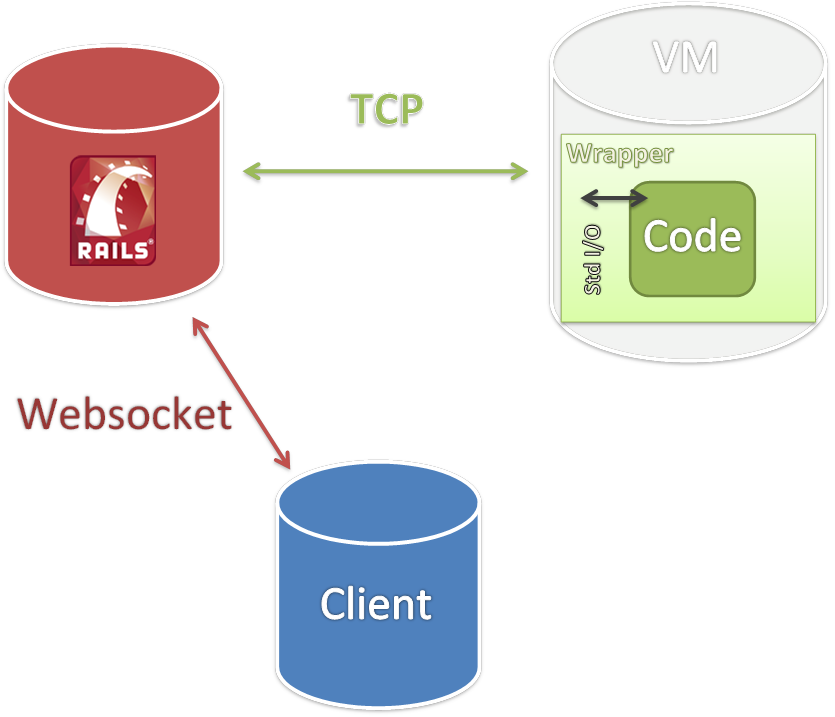
\includegraphics[scale=0.35]{overview}
\end{center}
\end{frame}

\begin{frame}
\frametitle{Javascript-Client}
\begin{center}
	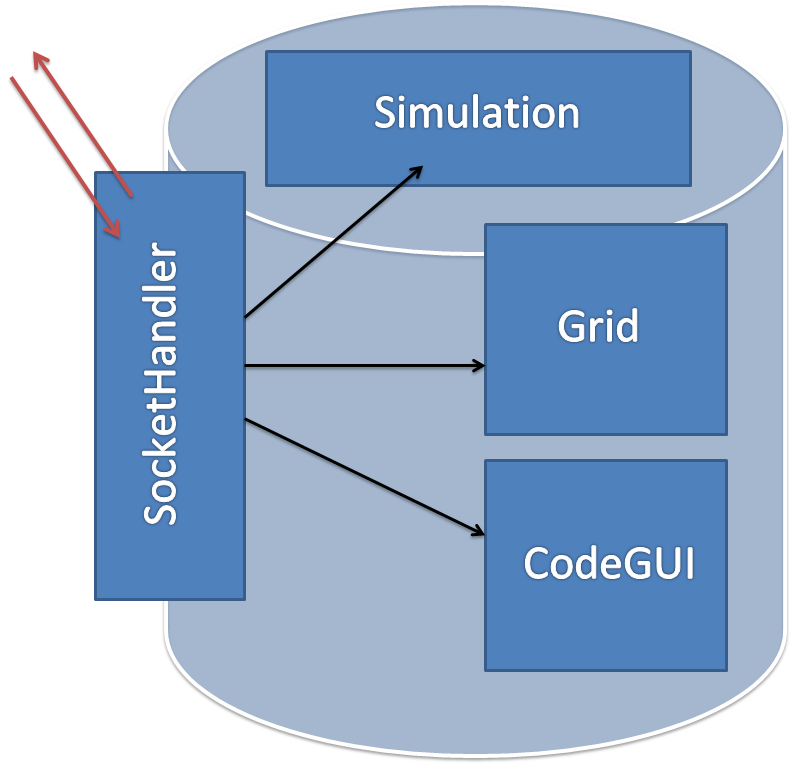
\includegraphics[scale=0.3]{client/modules.png}
\end{center}
\end{frame}

\begin{frame}
\frametitle{CodeGUI}
\begin{center}
	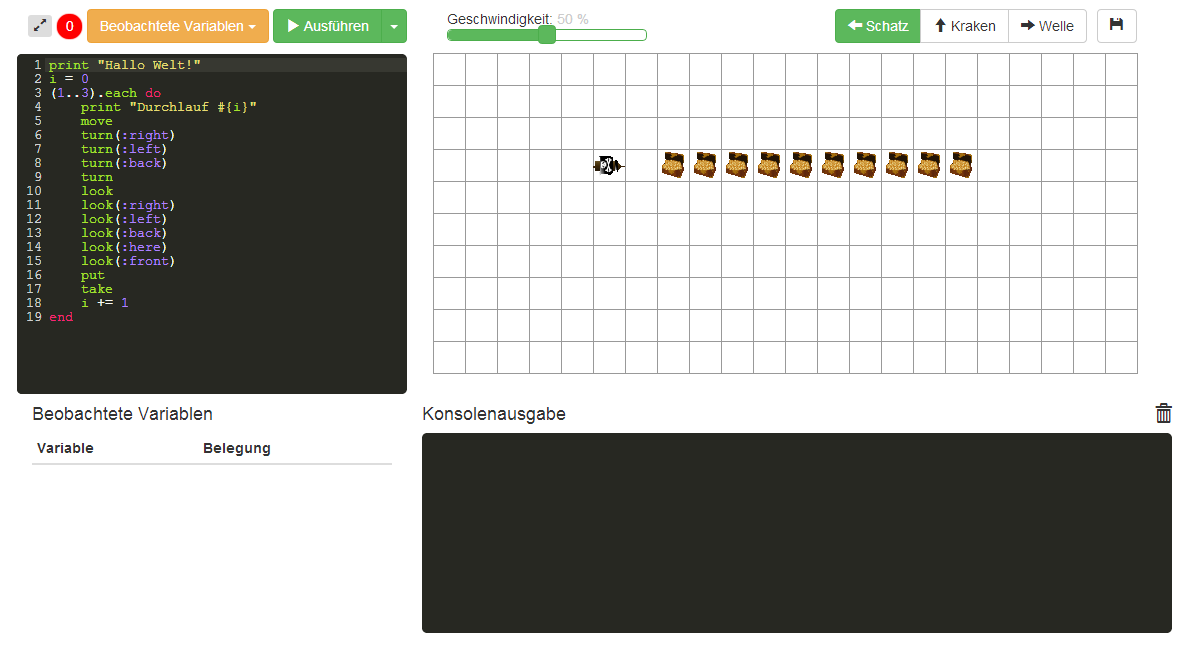
\includegraphics[scale=0.35]{client/client}
\end{center}
\end{frame}

\begin{frame}
\frametitle{SocketHandler}
	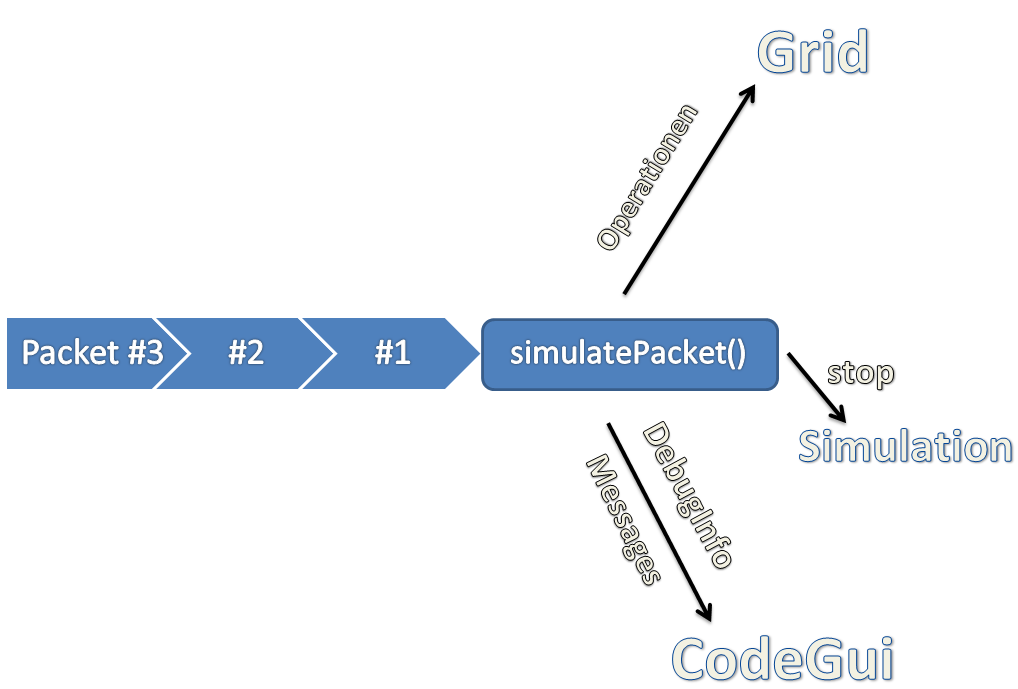
\includegraphics[scale=0.37]{client/socket-queue.PNG}
\end{frame}

\begin{frame}
\frametitle{SocketHandler}
\inputminted[linenos, numbersep=2pt, tabsize=4, frame=lines, label=Beispiel Paket]{json}{client/packet.json}
\end{frame}